% ==============================================================================
% SECAO 4 — CONTROLE PROPORCIONAL, ROUTH-HURWITZ E LGR
% ==============================================================================
\section{CONTROLE PROPORCIONAL, ROUTH-HURWITZ E LUGAR GEOMÉTRICO DAS RAÍZES}\label{sec:controle_p}

Como a malha aberta não regula a fila em patamar finito (Seção~\ref{sec:malha_aberta}), introduz-se a realimentação unitária negativa com um controlador proporcional $C_P(s) = K$, cujas estabilidade, dinâmica modal, precisão estacionária e limitações são examinadas a seguir.

\subsection{Função de Transferência em Malha Fechada e Equação Característica}\label{sec:ft_mf_p}
Adotando realimentação unitária negativa ($E(s) = X_r(s) - X(s)$) e um controlador proporcional puro $C_P(s) = K$, a função de transferência de ramo direto é $L_P(s) = K G(s) = \frac{K}{s(2s+1)}$. A função de transferência em malha fechada para referência é:
\begin{equation}
    T_P(s) = \frac{X(s)}{X_r(s)} = \frac{K G(s)}{1 + K G(s)} = \frac{K}{2s^2 + s + K} = \frac{K/2}{s^2 + 0{,}5s + K/2}.
    \label{eq:ft_mf_p}
\end{equation}
Para a perturbação de chegada $\Delta\Lambda(s)$ (com $X_r(s)=0$), o diagrama da Figura~\ref{fig:diagrama_blocos} fornece:
\begin{equation}
    T_{d,P}(s) = \frac{X(s)}{\Delta\Lambda(s)} = -\frac{2s + 1}{2s^2 + s + K}.
    \label{eq:ft_dist_p}
\end{equation}
A equação característica do sistema em malha fechada é dada pelo denominador comum:
\begin{equation}
    2s^2 + s + K = 0 \qquad \Longleftrightarrow \qquad s^2 + 0{,}5s + \frac{K}{2} = 0.
    \label{eq:ec_p}
\end{equation}

\subsection{Critério de Routh-Hurwitz e Estabilidade Assintótica}\label{sec:routh_p}
Aplicando o critério de Routh-Hurwitz ao polinômio característico $P(s) = 2s^2 + s + K$ (OGATA, 2010; NISE, 2017), constrói-se o arranjo tabular:
\[
\begin{array}{c|cc}
    s^2 & 2 & K \\
    s^1 & 1 & 0 \\
    s^0 & K & 0
\end{array}
\]
A estabilidade assintótica exige que todos os elementos da primeira coluna do arranjo de Routh sejam estritamente positivos ($2 > 0$, $1 > 0$ e $K > 0$). Logo, o sistema em malha fechada linear é assintoticamente estável para todo:
\begin{equation}
    K > 0.
\end{equation}

\subsection{Condição para Resposta Não Oscilatória e Assintoticamente Estável}\label{sec:nao_osc_p}
As raízes da Equação~\eqref{eq:ec_p} são:
\begin{equation}
    s_{1,2} = \frac{-1 \pm \sqrt{1 - 8K}}{4} = -0{,}25 \pm \frac{\sqrt{1 - 8K}}{4}.
\end{equation}
Para que a resposta ao degrau seja não oscilatória (polos reais) e assintoticamente estável (polos no semiplano esquerdo aberto), o discriminante deve ser não negativo ($\Delta = 1 - 8K \ge 0$) junto com a condição $K > 0$. Portanto, existe faixa válida dada por:
\begin{equation}
    0 < K \le \frac{1}{8} = 0{,}125.
\end{equation}
Em particular, $0 < K < 0{,}125$ gera resposta sobreamortecida (dois polos reais negativos distintos) e $K = 0{,}125$ gera resposta criticamente amortecida (polo duplo em $s = -0{,}25\text{ s}^{-1}$).

\subsection{Influência de $K$ sobre Polos, Frequência Natural, Amortecimento e Velocidade}\label{sec:influencia_k}
Comparando $s^2 + 0{,}5s + 0{,}5K = 0$ com a forma canônica de segunda ordem $s^2 + 2\zeta\omega_n s + \omega_n^2 = 0$ (DORF; BISHOP, 2018), obtém-se explicitamente:
\begin{equation}
    \omega_n(K) = \sqrt{\frac{K}{2}}, \qquad \zeta(K) = \frac{0{,}5}{2\omega_n} = \frac{1}{\sqrt{8K}}, \qquad \sigma = -\zeta\omega_n = -0{,}25\text{ s}^{-1} \quad (\text{para } K \ge 0{,}125).
    \label{eq:wn_zeta_p}
\end{equation}
Dessas relações decorrem as principais consequências para o regime transitório. Primeiramente, a frequência natural $\omega_n$ cresce proporcionalmente a $\sqrt{K}$, ampliando a largura de banda e reduzindo o tempo de subida $t_r$ à medida que o ganho aumenta. Em contrapartida, o fator de amortecimento $\zeta$ decresce na razão inversa $1/\sqrt{K}$; assim, para todo $K > 0{,}125$, tem-se $\zeta < 1$ (regime subamortecido), resultando em sobressinal $M_p = \exp\!\left(-\pi\zeta/\sqrt{1-\zeta^2}\right)$ monotonicamente crescente com $K$.

Observa-se ainda uma restrição estrutural na parte real dos polos complexos: para todo $K \ge 0{,}125$, as raízes deslocam-se verticalmente ao longo da reta $\operatorname{Re}(s) = \sigma = -0{,}25\text{ s}^{-1}$, com frequência amortecida $\omega_d = \sqrt{0{,}5K - 0{,}0625}$. Disso resulta que o envelope exponencial $e^{-0{,}25t}$ é invariante com $K$, impondo um limite intrínseco à velocidade de acomodação ($t_s(2\%) \approx 4/|\sigma| \approx 16\text{ s}$, estimativa pelo envelope; na varredura de $0{,}21 \le K \le 2{,}0$, os tempos simulados situam-se entre $12{,}22$ e $17{,}24\text{ s}$, sendo $13{,}752\text{ s}$ em $K = 0{,}369$ e $14{,}118\text{ s}$ em $K = 2{,}0$). Por outro lado, tentar evitar oscilações operando no regime sobreamortecido ($0 < K < 0{,}125$) desloca o polo dominante $s_1 = -0{,}25 + \frac{1}{4}\sqrt{1-8K}$ em direção à origem quando $K \to 0^+$, tornando a resposta ainda mais lenta ($t_s \gg 16\text{ s}$).

\subsection{Limitações do Controlador Proporcional na Regulação e Rejeição a Perturbações}\label{sec:limitacoes_p}
Pelo Teorema do Valor Final (TVF), sob taxa de chegada nominal ($\Delta\lambda = 0$) e referência em degrau $X_r(s) = 300/s$:
\begin{equation}
    e_{ss,\text{ref}} = \lim_{s\to 0} s \cdot \frac{1}{1 + K G(s)} \frac{300}{s} = \lim_{s\to 0} \frac{s(2s+1)}{2s^2 + s + K}\,300 = 0,
\end{equation}
pois a própria planta possui um integrador (Tipo~1) (NISE, 2017). Contudo, quando ocorre a perturbação permanente em degrau $\Delta\lambda(t) = 100\,\mathbb{1}(t - 20)$ ($\Delta\Lambda(s) = 100/s$), a parcela de perturbação na Equação~\eqref{eq:ft_dist_p} produz em regime permanente:
\begin{equation}
    x_{ss,\text{dist}} = \lim_{s\to 0} s \left(-\frac{2s+1}{2s^2+s+K}\right)\frac{100}{s} = -\frac{100}{K}
    \implies e_{ss,\text{dist}} = \frac{100}{K}\text{ eventos}.
    \label{eq:ess_dist_p}
\end{equation}
Fisicamente, manter a fila estacionária ($\dot{q}=0$) sob $\lambda = 1100\text{ eventos/s}$ exige que a capacidade efetiva suba para $\mu_{ss} = 1100\text{ eventos/s}$ ($u_{ss} = +100$). Como o controlador proporcional só gera sinal de controle proporcional ao erro ($u_{ss} = K e_{ss}$), um erro estacionário não nulo $e_{ss} = 100/K$ é indispensável para sustentar o esforço $u_{ss}=100$. Para atender ao requisito $e_{ss} \le 10\text{ eventos}$, seria necessário $K \ge 10$, o que acarreta oscilações severas ($\zeta \le 0{,}112$, $M_p \ge 70\%$) e esforço de controle inicial irrealizável ($u(0^+) = 300K \ge 3000 \gg 400$).

\subsection{Lugar Geométrico das Raízes (LGR) da Planta com Controle P}\label{sec:lgr_p}
Considerando a equação característica paramétrica $1 + K G(s) = 1 + \frac{K}{s(2s+1)} = 0$, as regras de Evans caracterizam integralmente o traçado do Lugar Geométrico das Raízes (OGATA, 2010). Partindo dos dois polos de malha aberta ($n=2$) em $p_1 = 0$ e $p_2 = -0{,}5\text{ s}^{-1}$ e na ausência de zeros finitos ($m=0$), o segmento real $[-0{,}5,\, 0]$ pertence ao LGR por possuir número ímpar de polos à sua direita. A condição de separação (\textit{breakaway}), obtida por $\frac{d}{ds}\left[-s(2s+1)\right] = -(4s+1) = 0$, ocorre exatamente em $s_b = -0{,}25\text{ s}^{-1}$ para $K_b = 0{,}125$. A partir desse ponto, os dois ramos seguem as $n-m=2$ assíntotas verticais de ângulos $\theta_a = \pm 90^\circ$ e centroide $\sigma_a = \frac{0 + (-0{,}5)}{2} = -0{,}25\text{ s}^{-1}$. Em síntese, à medida que $K$ cresce em $(0,\,0{,}125)$, os polos reais convergem de $0$ e $-0{,}5$ até coincidirem em $-0{,}25$ e, para $K > 0{,}125$, afastam-se simetricamente em direção a $-0{,}25 \pm j\infty$.

Para ilustrar os distintos regimes dinâmicos ao longo desses ramos, selecionam-se quatro valores positivos de ganho: $K \in \{0{,}08,\, 0{,}125,\, 0{,}369,\, 2{,}0\}$, cujos polos, parâmetros modais e comportamento físico na fila são resumidos na Tabela~\ref{tab:polos_p} e visualizados nas Figuras~\ref{fig:lgr_p} e~\ref{fig:temporal_p}. O valor $K = 0{,}369$ corresponde ao ajuste no entorno de $M_p \approx 10\%$ adotado como referência para o controlador P.

\begin{table}[H]
\centering
\caption{Polos de malha fechada e comportamento dinâmico do controlador P para quatro valores de ganho $K$}
\label{tab:polos_p}
{\small\singlespacing
\resizebox{\textwidth}{!}{%
\begin{tabular}{ccccccl}
\toprule
\textbf{$K$} & \textbf{Polos $s_{1,2}$ ($\text{s}^{-1}$)} & \textbf{$\omega_n$ (rad/s)} & \textbf{$\zeta$} & \textbf{Regime} & \textbf{$e_{ss,\text{dist}}$ (eventos)} & \textbf{Comportamento de $q(t)$} \\
\midrule
$0{,}080$ & $-0{,}100,\; -0{,}400$ & $0{,}200$ & $1{,}250$ & Sobreamortecido & $1250{,}0$ & Lento, sem oscilação \\
$0{,}125$ & $-0{,}250,\; -0{,}250$ & $0{,}250$ & $1{,}000$ & Criticamente amortecido & $800{,}0$ & Mais rápido sem sobressinal \\
$0{,}369$ & $-0{,}250 \pm j\,0{,}349$ & $0{,}430$ & $0{,}582$ & Subamortecido (ref.) & $271{,}0$ & Pequeno sobressinal ($\approx 10{,}6\%$) \\
$2{,}000$ & $-0{,}250 \pm j\,0{,}968$ & $1{,}000$ & $0{,}250$ & Fortemente oscilatório & $50{,}0$ & Oscilações acentuadas ($\approx 44{,}4\%$) \\
\bottomrule
\end{tabular}%
}}
\fontefig{Fonte: Elaborada pelos autores com base nos resultados de simulação (2026).}
\end{table}

\begin{figure}[H]
\centering
\caption{Análise do controlador proporcional para $K \in \{0{,}08,\, 0{,}125,\, 0{,}369,\, 2{,}0\}$: (a) Lugar Geométrico das Raízes e (b) efeito dos polos sobre a velocidade e as oscilações da fila}
\label{fig:p_lgr_temporal}
\begin{subfigure}[b]{0.47\textwidth}
    \centering
    \IfFileExists{figuras/fig2_lgr_proporcional.pdf}{%
        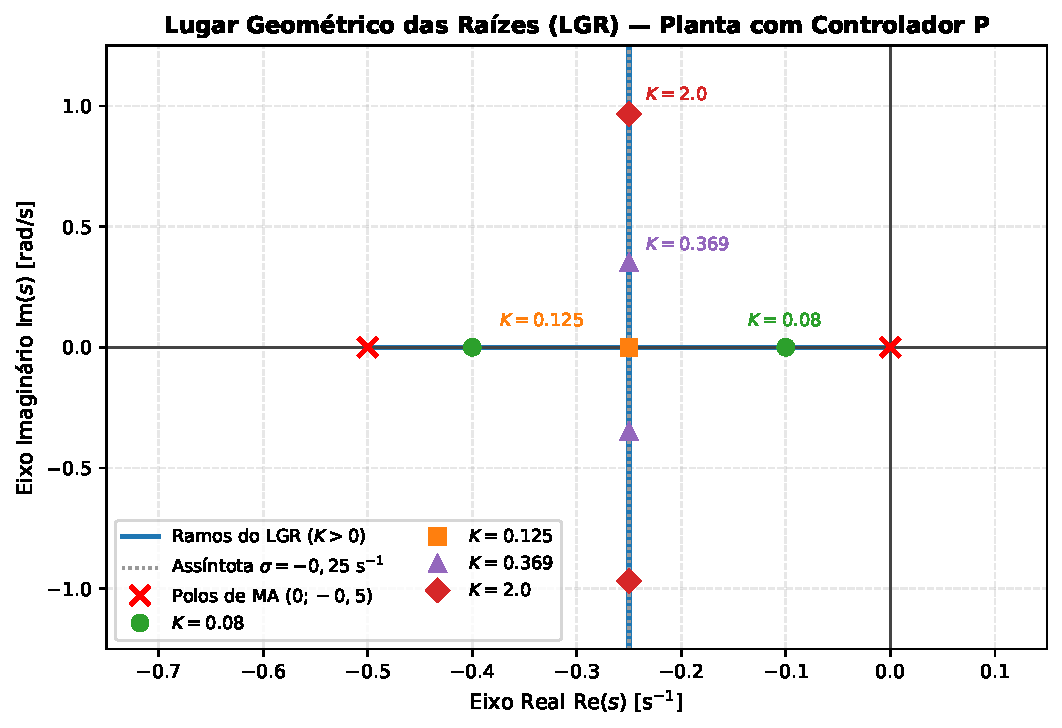
\includegraphics[width=\textwidth]{figuras/fig2_lgr_proporcional.pdf}%
    }{%
        \fbox{\parbox{0.9\textwidth}{\centering\vspace{1.0cm}\textit{[Aguardando \texttt{fig2\_lgr\_proporcional.pdf}]}\vspace{1.0cm}}}%
    }
    \caption{LGR da planta com controle P e polos para os quatro valores de $K$.}
    \label{fig:lgr_p}
\end{subfigure}
\hfill
\begin{subfigure}[b]{0.47\textwidth}
    \centering
    \IfFileExists{figuras/fig3_temporal_proporcional.pdf}{%
        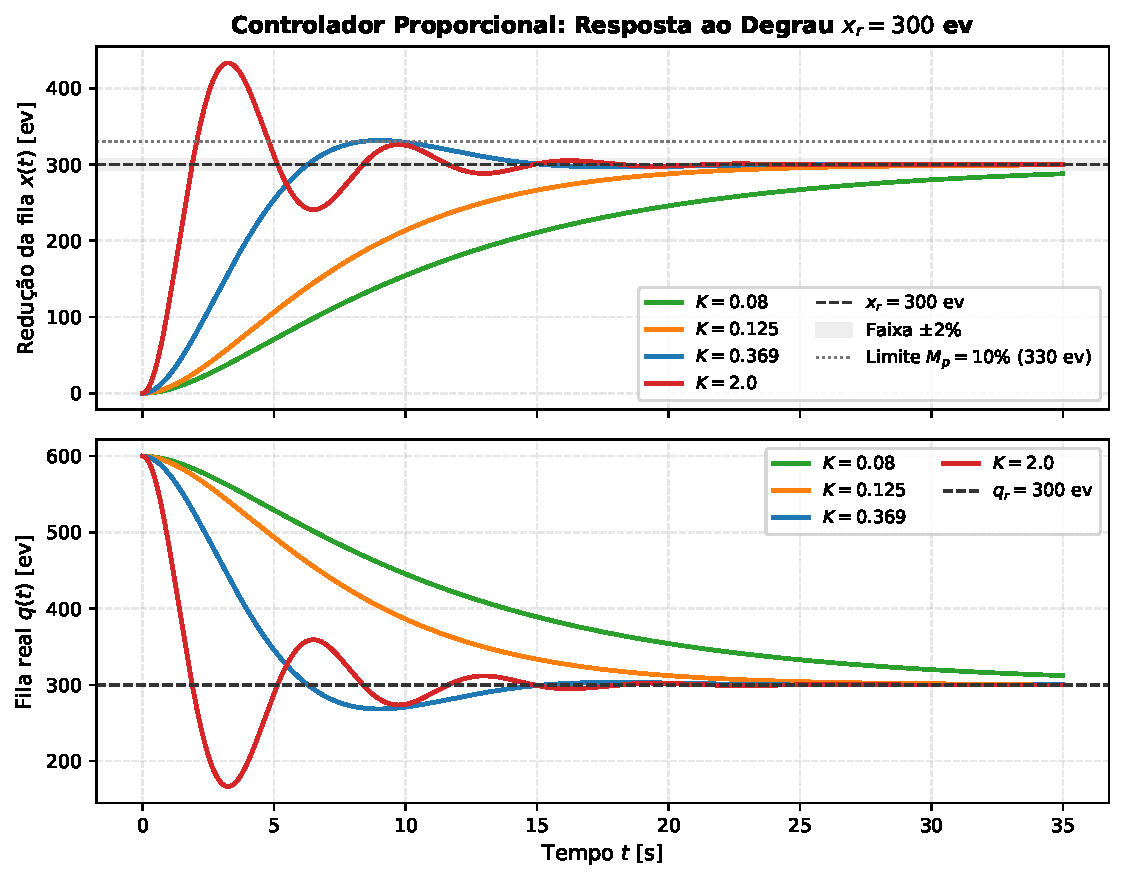
\includegraphics[width=\textwidth]{figuras/fig3_temporal_proporcional.pdf}%
    }{%
        \fbox{\parbox{0.9\textwidth}{\centering\vspace{1.0cm}\textit{[Aguardando \texttt{fig3\_temporal\_proporcional.pdf}]}\vspace{1.0cm}}}%
    }
    \caption{Respostas temporais de $x(t)$ e $q(t)$ para os quatro valores de $K$.}
    \label{fig:temporal_p}
\end{subfigure}
\fontefig{Fonte: Elaborada pelos autores com base nos resultados de simulação (2026).}
\end{figure}

\subsection{Impossibilidade de Atendimento Simultâneo dos Requisitos via Ajuste de $K$}\label{sec:impossibilidade_p}
As Equações~\eqref{eq:wn_zeta_p} e \eqref{eq:ess_dist_p} mostram que o ajuste exclusivo de $K$ não atende ao conjunto de requisitos. Como a parte real dos polos complexos fica fixa em $-0{,}25\text{ s}^{-1}$, o tempo de subida e o tempo de acomodação não podem ser reduzidos ao mesmo tempo: $t_r \le 5\text{ s}$ exige $K \gtrsim 0{,}31$, faixa em que $t_s$ permanece entre $12{,}22$ e $16{,}26\text{ s}$ (no ganho de referência $K = 0{,}369$, $t_s = 13{,}752\text{ s}$); o atendimento de $t_s \le 12\text{ s}$ ocorre apenas na faixa estreita $0{,}196 \lesssim K \lesssim 0{,}205$, na qual o sobressinal fica abaixo de $2\%$, mas $t_r$ permanece entre $7{,}48$ e $7{,}86\text{ s}$. Já o limite $M_p \le 10\%$ impõe $\zeta \ge 0{,}591$, isto é, $K \le 0{,}358$. Por fim, o requisito $e_{ss,\text{dist}} \le 10\text{ eventos}$ exige $K \ge 10$, valor cerca de $28$ vezes superior a esse limite, para o qual a margem de fase cai abaixo de $13^\circ$, o sobressinal supera $70\%$ e a capacidade solicitada excede o limite de $1400\text{ eventos/s}$. O controle puramente proporcional é, portanto, insuficiente, o que motiva a introdução das ações integral e derivativa na Seção~\ref{sec:projeto_comp}.
